% core TikZ only; no extra library beyond the paper preamble is required.
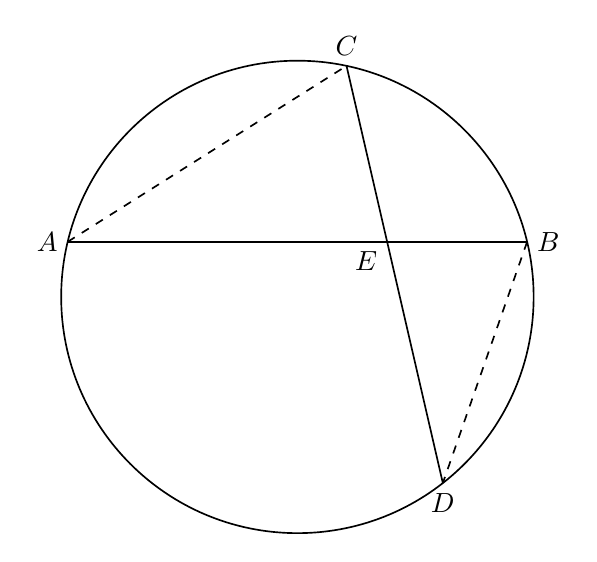
\begin{tikzpicture}[x=1cm,y=1cm,line width=.6pt,font=\normalsize]
\coordinate (A) at (-2.91719,0.7);
\coordinate (B) at (2.91719,0.7);
\coordinate (C) at (0.623735,2.934443);
\coordinate (D) at (1.846984,-2.364032);
\coordinate (E) at (1.139597,0.7);
\draw (0,0) circle[radius=3cm];
\draw (A)--(B);
\draw (C)--(D);
\draw[dashed] (A)--(C);
\draw[dashed] (B)--(D);
\node[left] at (A) {$A$};
\node[right] at (B) {$B$};
\node[above] at (C) {$C$};
\node[below] at (D) {$D$};
\node[below left] at (E) {$E$};
\end{tikzpicture}
